\documentclass{standalone}
\usepackage{tikz}
\usetikzlibrary{patterns, positioning}


\begin{document}
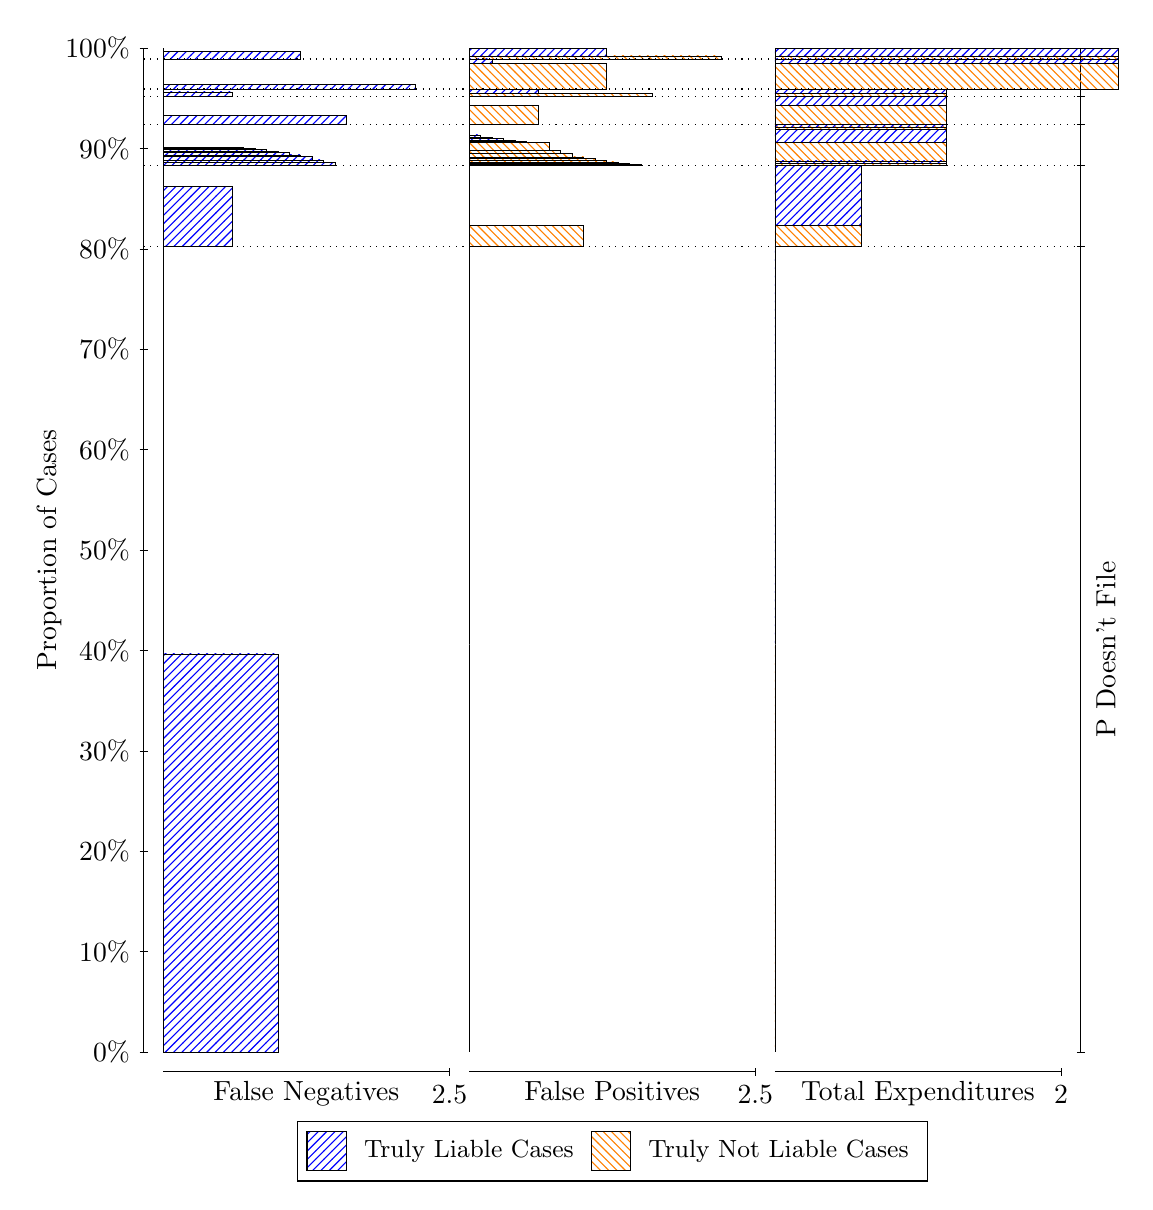
\begin{tikzpicture}
\draw[black, very thin] (1.5,1.75) -- (1.5,14.5);
\node[rotate=90, text=black, anchor=center] at (0.3, 8.125) {Proportion of Cases};
\draw[black, very thin] (1.45,1.75) -- (1.55,1.75);
\node[text=black, anchor=east] at (1.45, 1.75) {0\%};
\draw[black, very thin] (1.45,3.025) -- (1.55,3.025);
\node[text=black, anchor=east] at (1.45, 3.025) {10\%};
\draw[black, very thin] (1.45,4.3) -- (1.55,4.3);
\node[text=black, anchor=east] at (1.45, 4.3) {20\%};
\draw[black, very thin] (1.45,5.575) -- (1.55,5.575);
\node[text=black, anchor=east] at (1.45, 5.575) {30\%};
\draw[black, very thin] (1.45,6.85) -- (1.55,6.85);
\node[text=black, anchor=east] at (1.45, 6.85) {40\%};
\draw[black, very thin] (1.45,8.125) -- (1.55,8.125);
\node[text=black, anchor=east] at (1.45, 8.125) {50\%};
\draw[black, very thin] (1.45,9.4) -- (1.55,9.4);
\node[text=black, anchor=east] at (1.45, 9.4) {60\%};
\draw[black, very thin] (1.45,10.675) -- (1.55,10.675);
\node[text=black, anchor=east] at (1.45, 10.675) {70\%};
\draw[black, very thin] (1.45,11.95) -- (1.55,11.95);
\node[text=black, anchor=east] at (1.45, 11.95) {80\%};
\draw[black, very thin] (1.45,13.225) -- (1.55,13.225);
\node[text=black, anchor=east] at (1.45, 13.225) {90\%};
\draw[black, very thin] (1.45,14.5) -- (1.55,14.5);
\node[text=black, anchor=east] at (1.45, 14.5) {100\%};

\draw[black, very thin] (13.4,1.75) -- (13.4,14.5);
\draw[black, very thin] (13.35,1.75) -- (13.45,1.75);
\node[anchor=west] at (13.35, 1.75) {};
\draw[black, very thin] (13.35,11.977) -- (13.45,11.977);
\node[anchor=west] at (13.35, 11.977) {};
\draw[black, very thin] (13.35,13.009) -- (13.45,13.009);
\node[anchor=west] at (13.35, 13.009) {};
\draw[black, very thin] (13.35,13.53) -- (13.45,13.53);
\node[anchor=west] at (13.35, 13.53) {};
\draw[black, very thin] (13.35,13.887) -- (13.45,13.887);
\node[anchor=west] at (13.35, 13.887) {};
\draw[black, very thin] (13.35,13.979) -- (13.45,13.979);
\node[anchor=west] at (13.35, 13.979) {};
\draw[black, very thin] (13.35,14.361) -- (13.45,14.361);
\node[anchor=west] at (13.35, 14.361) {};
\draw[black, very thin] (13.35,14.5) -- (13.45,14.5);
\node[anchor=west] at (13.35, 14.5) {};

\draw[black, very thin, pattern color=blue, pattern=north east lines] (1.75,1.75) rectangle (3.2033,6.8052);
\draw[black, very thin, pattern color=orange, pattern=north west lines] (1.75,6.8052) rectangle (1.75,11.977);
\draw[black, very thin, pattern color=blue, pattern=north east lines] (1.75,11.977) rectangle (2.622,12.742);
\draw[black, very thin, pattern color=orange, pattern=north west lines] (1.75,12.742) rectangle (1.75,13.009);
\draw[black, very thin, pattern color=blue, pattern=north east lines] (1.75,13.009) rectangle (3.93,13.048);
\draw[black, very thin, pattern color=blue, pattern=north east lines] (1.75,13.048) rectangle (3.7847,13.079);
\draw[black, very thin, pattern color=blue, pattern=north east lines] (1.75,13.079) rectangle (3.6393,13.124);
\draw[black, very thin, pattern color=blue, pattern=north east lines] (1.75,13.124) rectangle (3.494,13.143);
\draw[black, very thin, pattern color=blue, pattern=north east lines] (1.75,13.143) rectangle (3.3487,13.172);
\draw[black, very thin, pattern color=blue, pattern=north east lines] (1.75,13.172) rectangle (3.2033,13.191);
\draw[black, very thin, pattern color=blue, pattern=north east lines] (1.75,13.191) rectangle (3.058,13.212);
\draw[black, very thin, pattern color=blue, pattern=north east lines] (1.75,13.212) rectangle (2.9127,13.223);
\draw[black, very thin, pattern color=blue, pattern=north east lines] (1.75,13.223) rectangle (2.7673,13.235);
\draw[black, very thin, pattern color=orange, pattern=north west lines] (1.75,13.235) rectangle (1.75,13.53);
\draw[black, very thin, pattern color=blue, pattern=north east lines] (1.75,13.53) rectangle (4.0753,13.643);
\draw[black, very thin, pattern color=orange, pattern=north west lines] (1.75,13.643) rectangle (1.75,13.887);
\draw[black, very thin, pattern color=blue, pattern=north east lines] (1.75,13.887) rectangle (2.622,13.943);
\draw[black, very thin, pattern color=orange, pattern=north west lines] (1.75,13.943) rectangle (1.75,13.979);
\draw[black, very thin, pattern color=blue, pattern=north east lines] (1.75,13.979) rectangle (4.9473,14.039);
\draw[black, very thin, pattern color=orange, pattern=north west lines] (1.75,14.039) rectangle (1.75,14.361);
\draw[black, very thin, pattern color=blue, pattern=north east lines] (1.75,14.361) rectangle (3.494,14.461);
\draw[black, very thin, pattern color=orange, pattern=north west lines] (1.75,14.461) rectangle (1.75,14.5);
\draw[black, very thin, pattern color=orange, pattern=north west lines] (5.6333,1.75) rectangle (5.6333,6.9223);
\draw[black, very thin, pattern color=blue, pattern=north east lines] (5.6333,6.9223) rectangle (5.6333,11.977);
\draw[black, very thin, pattern color=orange, pattern=north west lines] (5.6333,11.977) rectangle (7.0867,12.245);
\draw[black, very thin, pattern color=blue, pattern=north east lines] (5.6333,12.245) rectangle (5.6333,13.009);
\draw[black, very thin, pattern color=orange, pattern=north west lines] (5.6333,13.009) rectangle (7.8133,13.021);
\draw[black, very thin, pattern color=orange, pattern=north west lines] (5.6333,13.021) rectangle (7.668,13.033);
\draw[black, very thin, pattern color=orange, pattern=north west lines] (5.6333,13.033) rectangle (7.5227,13.053);
\draw[black, very thin, pattern color=orange, pattern=north west lines] (5.6333,13.053) rectangle (7.3773,13.072);
\draw[black, very thin, pattern color=orange, pattern=north west lines] (5.6333,13.072) rectangle (7.232,13.1);
\draw[black, very thin, pattern color=orange, pattern=north west lines] (5.6333,13.1) rectangle (7.0867,13.118);
\draw[black, very thin, pattern color=orange, pattern=north west lines] (5.6333,13.118) rectangle (6.9413,13.164);
\draw[black, very thin, pattern color=orange, pattern=north west lines] (5.6333,13.164) rectangle (6.796,13.199);
\draw[black, very thin, pattern color=orange, pattern=north west lines] (5.6333,13.199) rectangle (6.6507,13.304);
\draw[black, very thin, pattern color=blue, pattern=north east lines] (5.6333,13.304) rectangle (6.36,13.316);
\draw[black, very thin, pattern color=blue, pattern=north east lines] (5.6333,13.316) rectangle (6.2147,13.327);
\draw[black, very thin, pattern color=blue, pattern=north east lines] (5.6333,13.327) rectangle (6.0693,13.348);
\draw[black, very thin, pattern color=blue, pattern=north east lines] (5.6333,13.348) rectangle (5.924,13.367);
\draw[black, very thin, pattern color=blue, pattern=north east lines] (5.6333,13.367) rectangle (5.7787,13.396);
\draw[black, very thin, pattern color=blue, pattern=north east lines] (5.6333,13.396) rectangle (5.6333,13.53);
\draw[black, very thin, pattern color=orange, pattern=north west lines] (5.6333,13.53) rectangle (6.5053,13.774);
\draw[black, very thin, pattern color=blue, pattern=north east lines] (5.6333,13.774) rectangle (5.6333,13.887);
\draw[black, very thin, pattern color=orange, pattern=north west lines] (5.6333,13.887) rectangle (7.9587,13.922);
\draw[black, very thin, pattern color=blue, pattern=north east lines] (5.6333,13.922) rectangle (6.5053,13.979);
\draw[black, very thin, pattern color=orange, pattern=north west lines] (5.6333,13.979) rectangle (7.3773,14.301);
\draw[black, very thin, pattern color=blue, pattern=north east lines] (5.6333,14.301) rectangle (5.924,14.361);
\draw[black, very thin, pattern color=orange, pattern=north west lines] (5.6333,14.361) rectangle (8.8307,14.401);
\draw[black, very thin, pattern color=blue, pattern=north east lines] (5.6333,14.401) rectangle (7.3773,14.5);
\draw[black, very thin, pattern color=orange, pattern=north west lines] (9.5167,1.75) rectangle (9.5167,6.9223);
\draw[black, very thin, pattern color=blue, pattern=north east lines] (9.5167,6.9223) rectangle (9.5167,11.977);
\draw[black, very thin, pattern color=orange, pattern=north west lines] (9.5167,11.977) rectangle (10.607,12.245);
\draw[black, very thin, pattern color=blue, pattern=north east lines] (9.5167,12.245) rectangle (10.607,13.009);
\draw[black, very thin, pattern color=orange, pattern=north west lines] (9.5167,13.009) rectangle (11.697,13.037);
\draw[black, very thin, pattern color=blue, pattern=north east lines] (9.5167,13.037) rectangle (11.697,13.066);
\draw[black, very thin, pattern color=orange, pattern=north west lines] (9.5167,13.066) rectangle (11.697,13.3);
\draw[black, very thin, pattern color=blue, pattern=north east lines] (9.5167,13.3) rectangle (11.697,13.465);
\draw[black, very thin, pattern color=orange, pattern=north west lines] (9.5167,13.465) rectangle (11.697,13.498);
\draw[black, very thin, pattern color=blue, pattern=north east lines] (9.5167,13.498) rectangle (11.697,13.53);
\draw[black, very thin, pattern color=orange, pattern=north west lines] (9.5167,13.53) rectangle (11.697,13.774);
\draw[black, very thin, pattern color=blue, pattern=north east lines] (9.5167,13.774) rectangle (11.697,13.887);
\draw[black, very thin, pattern color=orange, pattern=north west lines] (9.5167,13.887) rectangle (11.697,13.922);
\draw[black, very thin, pattern color=blue, pattern=north east lines] (9.5167,13.922) rectangle (11.697,13.979);
\draw[black, very thin, pattern color=orange, pattern=north west lines] (9.5167,13.979) rectangle (13.877,14.301);
\draw[black, very thin, pattern color=blue, pattern=north east lines] (9.5167,14.301) rectangle (13.877,14.361);
\draw[black, very thin, pattern color=orange, pattern=north west lines] (9.5167,14.361) rectangle (13.877,14.401);
\draw[black, very thin, pattern color=blue, pattern=north east lines] (9.5167,14.401) rectangle (13.877,14.5);
\draw[black, dotted] (1.5,11.977) -- (13.4,11.977);
\draw[black, dotted] (1.5,13.009) -- (13.4,13.009);
\draw[black, dotted] (1.5,13.53) -- (13.4,13.53);
\draw[black, dotted] (1.5,13.887) -- (13.4,13.887);
\draw[black, dotted] (1.5,13.979) -- (13.4,13.979);
\draw[black, dotted] (1.5,14.361) -- (13.4,14.361);
\draw[black, very thin] (1.75,1.5) -- (5.3833,1.5);
\node[text=black, anchor=north] at (3.5667, 1.5) {False Negatives};
\draw[black, very thin] (5.3833,1.45) -- (5.3833,1.55);
\node[text=black, anchor=north] at (5.3833, 1.45) {2.5};

\draw[black, very thin] (5.6333,1.5) -- (9.2667,1.5);
\node[text=black, anchor=north] at (7.45, 1.5) {False Positives};
\draw[black, very thin] (9.2667,1.45) -- (9.2667,1.55);
\node[text=black, anchor=north] at (9.2667, 1.45) {2.5};

\draw[black, very thin] (9.5167,1.5) -- (13.15,1.5);
\node[text=black, anchor=north] at (11.333, 1.5) {Total Expenditures};
\draw[black, very thin] (13.15,1.45) -- (13.15,1.55);
\node[text=black, anchor=north] at (13.15, 1.45) {2};

\node[text=black, centered, rotate=90] at (13.72, 6.8637) {P Doesn't File};







\draw (7.449999999999999,1.5) node[draw=none] (baseCoordinate) {};
\begin{scope}[align=center]
        \matrix[scale=0.5, draw=black, below=0.5cm of baseCoordinate, nodes={draw}, column sep=0.1cm]{
            \node[rectangle, draw, minimum width=0.5cm, minimum height=0.5cm, pattern color=blue, pattern=north east lines] {}; &
            \node[draw=none, font=\small, text=black] (B) {Truly Liable Cases}; &
            \node[rectangle, draw, minimum width=0.5cm, minimum height=0.5cm, pattern color=orange, pattern=north west lines] {}; &
            \node[draw=none, font=\small, text=black] (B) {Truly Not Liable Cases}; \\
            };
\end{scope}

\end{tikzpicture}
\end{document}